\documentclass[11pt]{ctexart}
\usepackage[margin=1in]{geometry}
\usepackage{graphicx}
\usepackage{booktabs}
\usepackage{amsmath}
\usepackage{hyperref}
\title{breakup g4output 上 RK 与 NN 质子重建对比 \\ \large 头对头评估}
\date{2026-06-18}
\begin{document}
\maketitle

\begin{abstract}
本报告评估 d+Sn breakup 样本 (ypol + zpol, 176 cells) 上两种后端的质子重建质量: RK (Runge-Kutta 最小二乘拟合器, three-point-free 模式, 在 spana03 上运行) 与 NN (6-128-128-64 MLP, formal\_B115T3deg/20260420\_184345 模型, 本地运行)。两套重建均来自同一 Geant4 g4output, 因此可以按事件 entry-index 一一对应。报告质子的三套误差 (RK-vs-truth, NN-vs-truth, RK-vs-NN), 以及中子的 truth-vs-reco 残差 (NEBULA $\beta$-method, 两种后端相同)。样本: 共 3301419 个 truth-proton 事件。
\end{abstract}

\section{数据与方法}
\textbf{RK reco}: spana03 \texttt{data/reconstruction/dbreak\_elastic/}, 176 文件, 2026-05-09 由 \texttt{run\_dbreak\_elastic\_pipeline.py stage\_reco} 产出 (\texttt{--backend rk --rk-fit-mode three-point-free --max-iterations 40})。\\
\textbf{NN reco}: 本地 \texttt{data/reconstruction/breakup\_nn\_20260503/}, 176 文件, 2026-05-03 由 \texttt{01\_run\_nn\_reco.sh} 产出 (clean production model \texttt{formal\_B115T3deg/20260420\_184345})。\\
\textbf{g4output}: 两种后端使用相同 g4output (已验证文件大小 285252607 字节, 时间戳 2026-05-01 20:16:46 +0900)。Per-event entry-index 1:1 对齐有效。\\
\textbf{参考系}: target frame (beam-as-Z)。truth 已是 target frame; 两种后端的 reco 在写入时由 \texttt{RotateRecoResultToTargetFrame} 旋转至 target frame (\texttt{apps/run\_reconstruction/main.cc:629-630})。本分析无需额外旋转。\\

\section{质子重建 --- RK vs NN vs truth}
\subsection{全局残差}
\begin{table}[h]\centering\small\begin{tabular}{lllll}\toprule
Pol & Backend & $\Delta p_x$ & $\Delta p_y$ & $\Delta p_z$ \\\midrule
ypol & RK & MAE=11.4, RMSE=39.7, Bias=-6.8, P95=30.7, N=2150443 & MAE=1.6, RMSE=3.5, Bias=-0.1, P95=4.1, N=2150443 & MAE=20.3, RMSE=87.8, Bias=-11.1, P95=26.8, N=2150443 \\
ypol & NN & MAE=6.1, RMSE=13.3, Bias=-1.8, P95=14.4, N=2150443 & MAE=1.3, RMSE=2.4, Bias=+0.5, P95=3.2, N=2150443 & MAE=6.6, RMSE=15.7, Bias=+2.8, P95=15.2, N=2150443 \\
zpol & RK & MAE=12.0, RMSE=46.8, Bias=-7.4, P95=35.3, N=101662 & MAE=1.7, RMSE=4.8, Bias=-0.2, P95=3.9, N=101662 & MAE=21.2, RMSE=91.8, Bias=-11.3, P95=30.8, N=101662 \\
zpol & NN & MAE=7.1, RMSE=13.7, Bias=-2.6, P95=22.2, N=101662 & MAE=1.4, RMSE=3.0, Bias=+0.6, P95=3.3, N=101662 & MAE=7.6, RMSE=15.5, Bias=+3.4, P95=23.8, N=101662 \\
\bottomrule\end{tabular}\end{table}
\begin{figure}[h]\centering
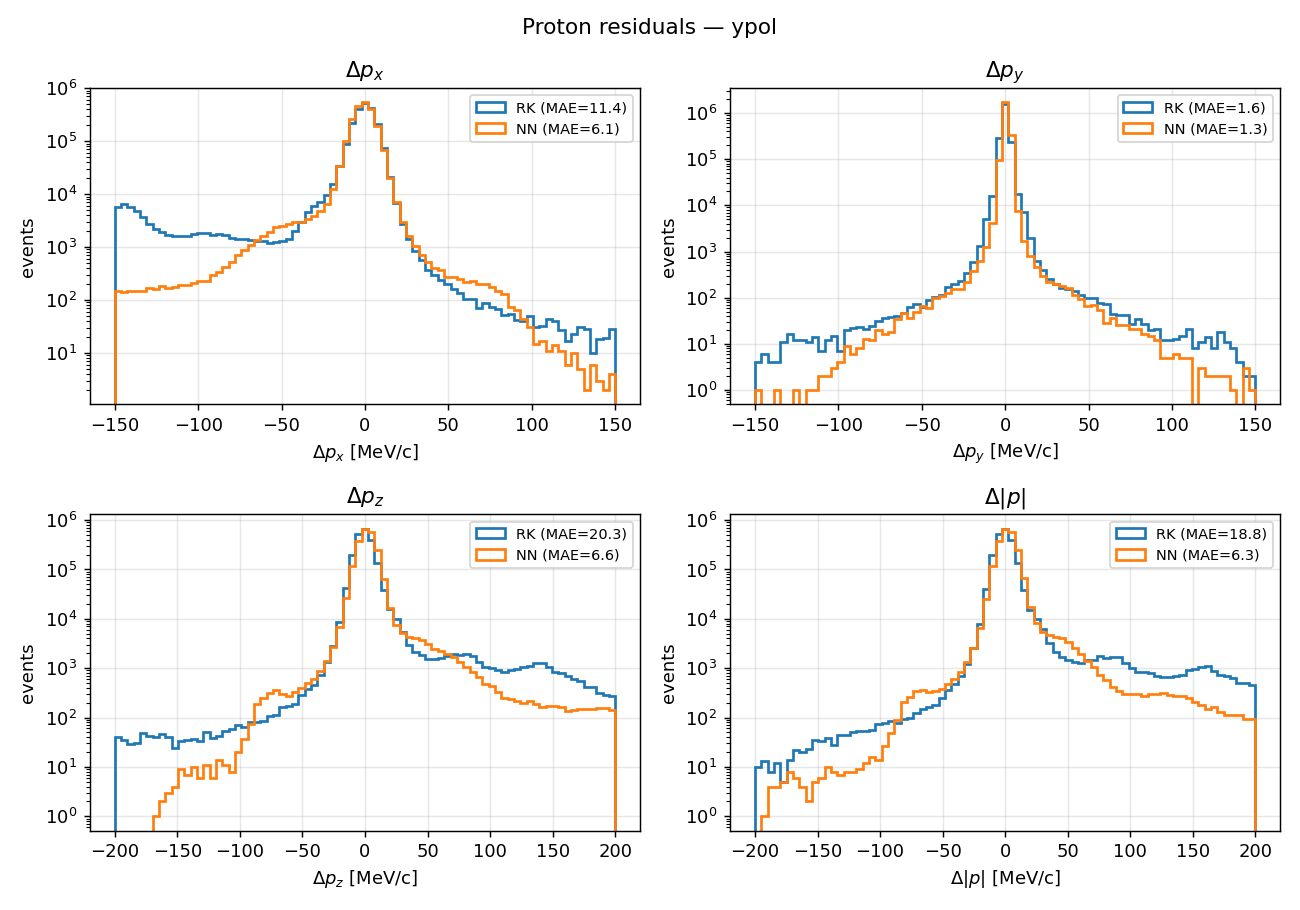
\includegraphics[width=0.95\textwidth]{figures/rk_vs_nn_breakup/proton_residuals_ypol.png}
\caption{质子残差分布, ypol。}
\end{figure}

\begin{figure}[h]\centering
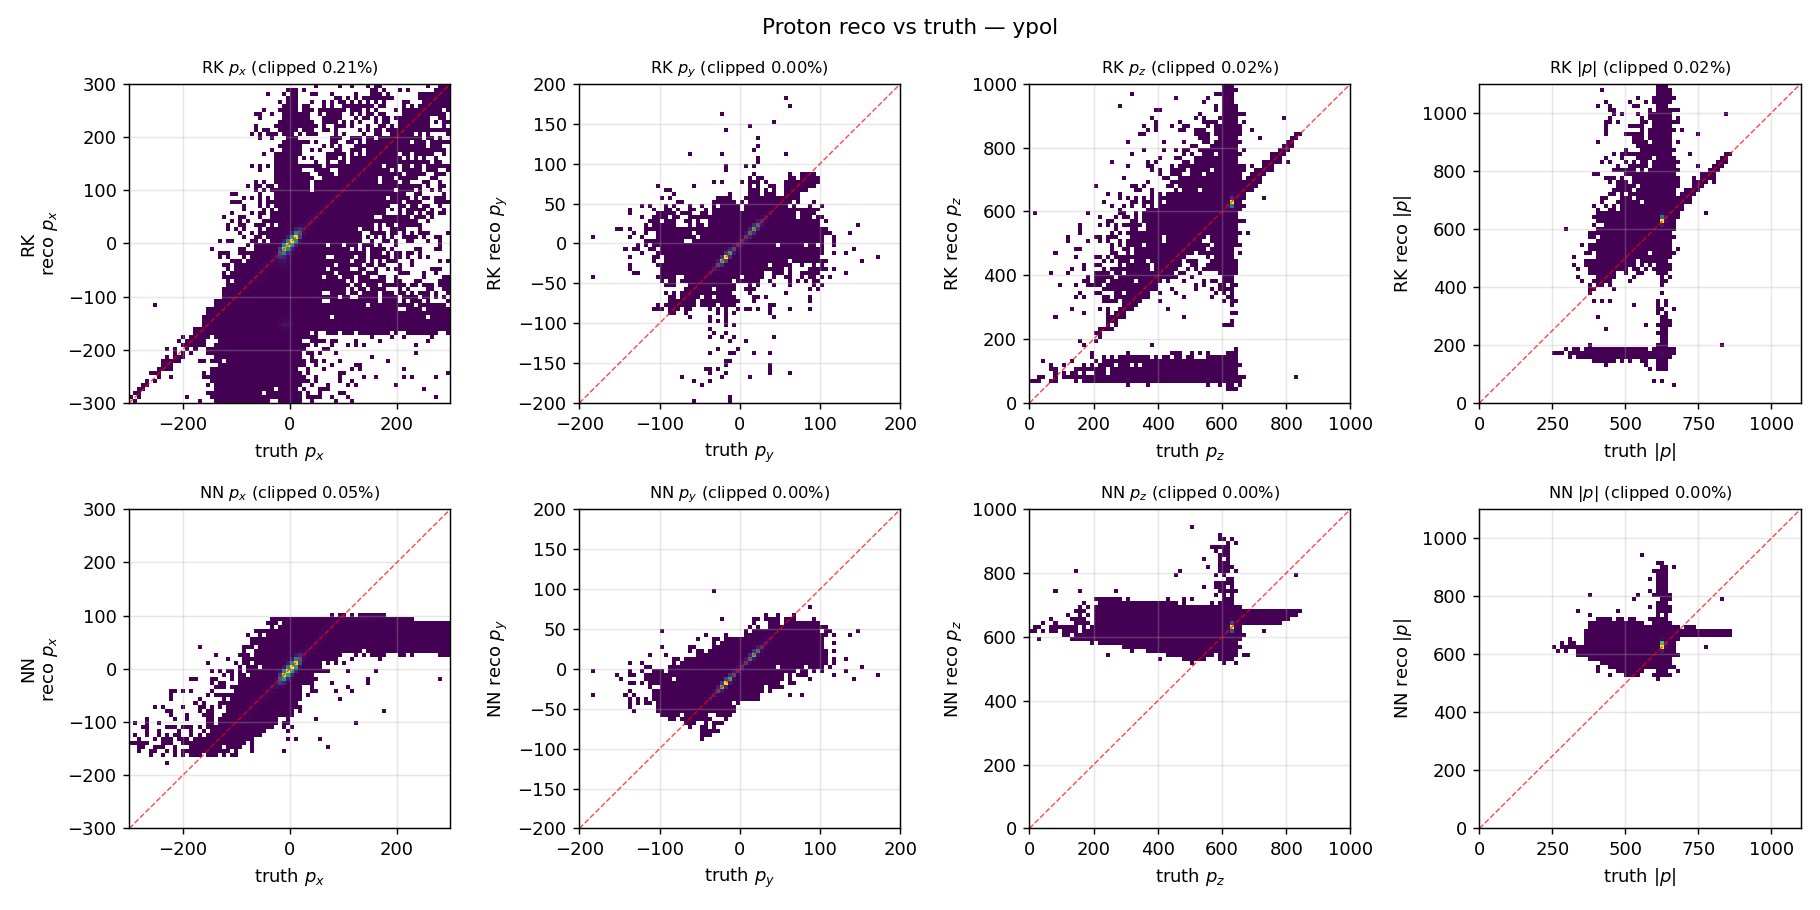
\includegraphics[width=0.95\textwidth]{figures/rk_vs_nn_breakup/proton_reco_vs_truth_ypol.png}
\caption{质子 reco vs truth 2D 散点, ypol。}
\end{figure}

\begin{figure}[h]\centering
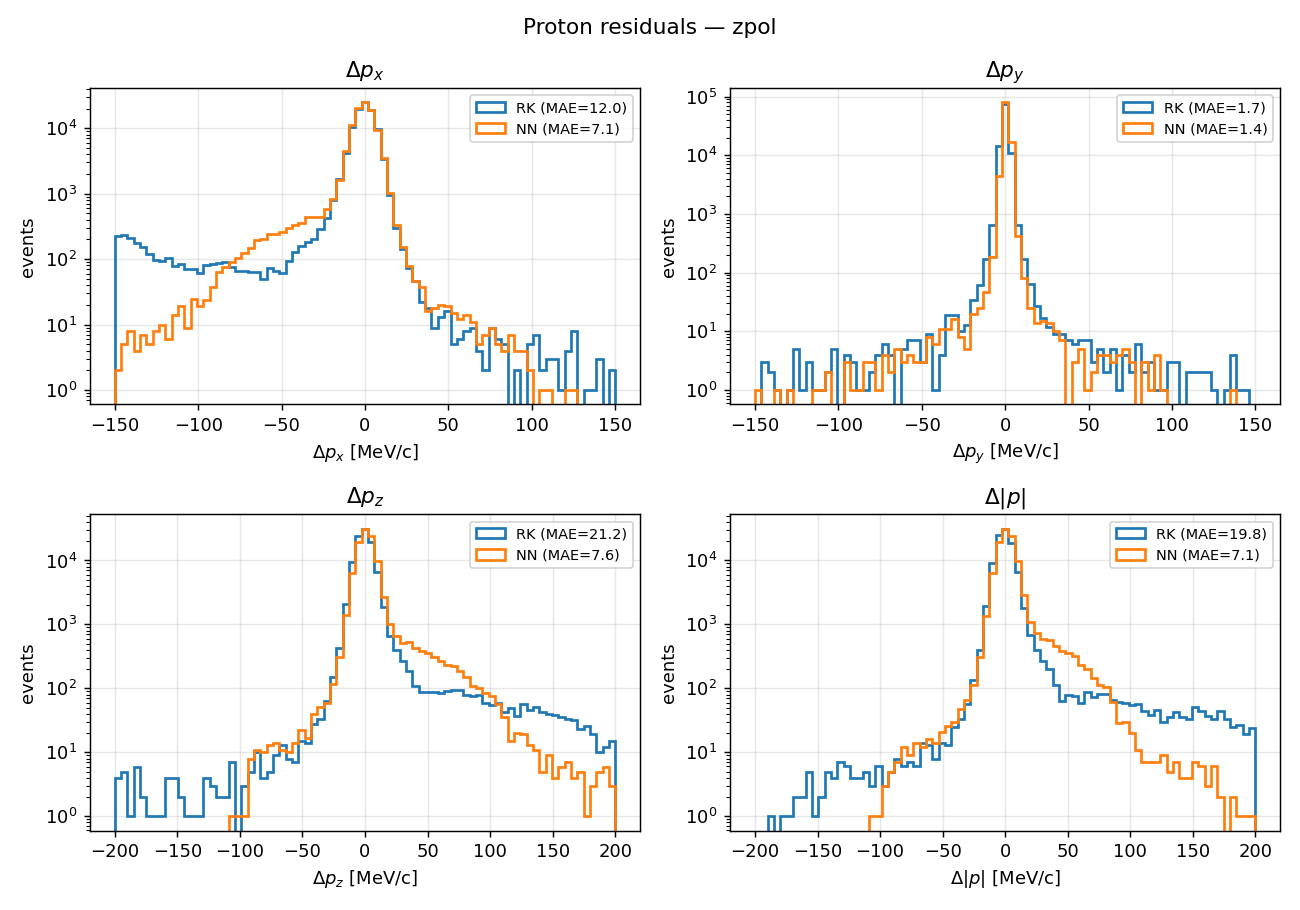
\includegraphics[width=0.95\textwidth]{figures/rk_vs_nn_breakup/proton_residuals_zpol.png}
\caption{质子残差分布, zpol。}
\end{figure}

\begin{figure}[h]\centering
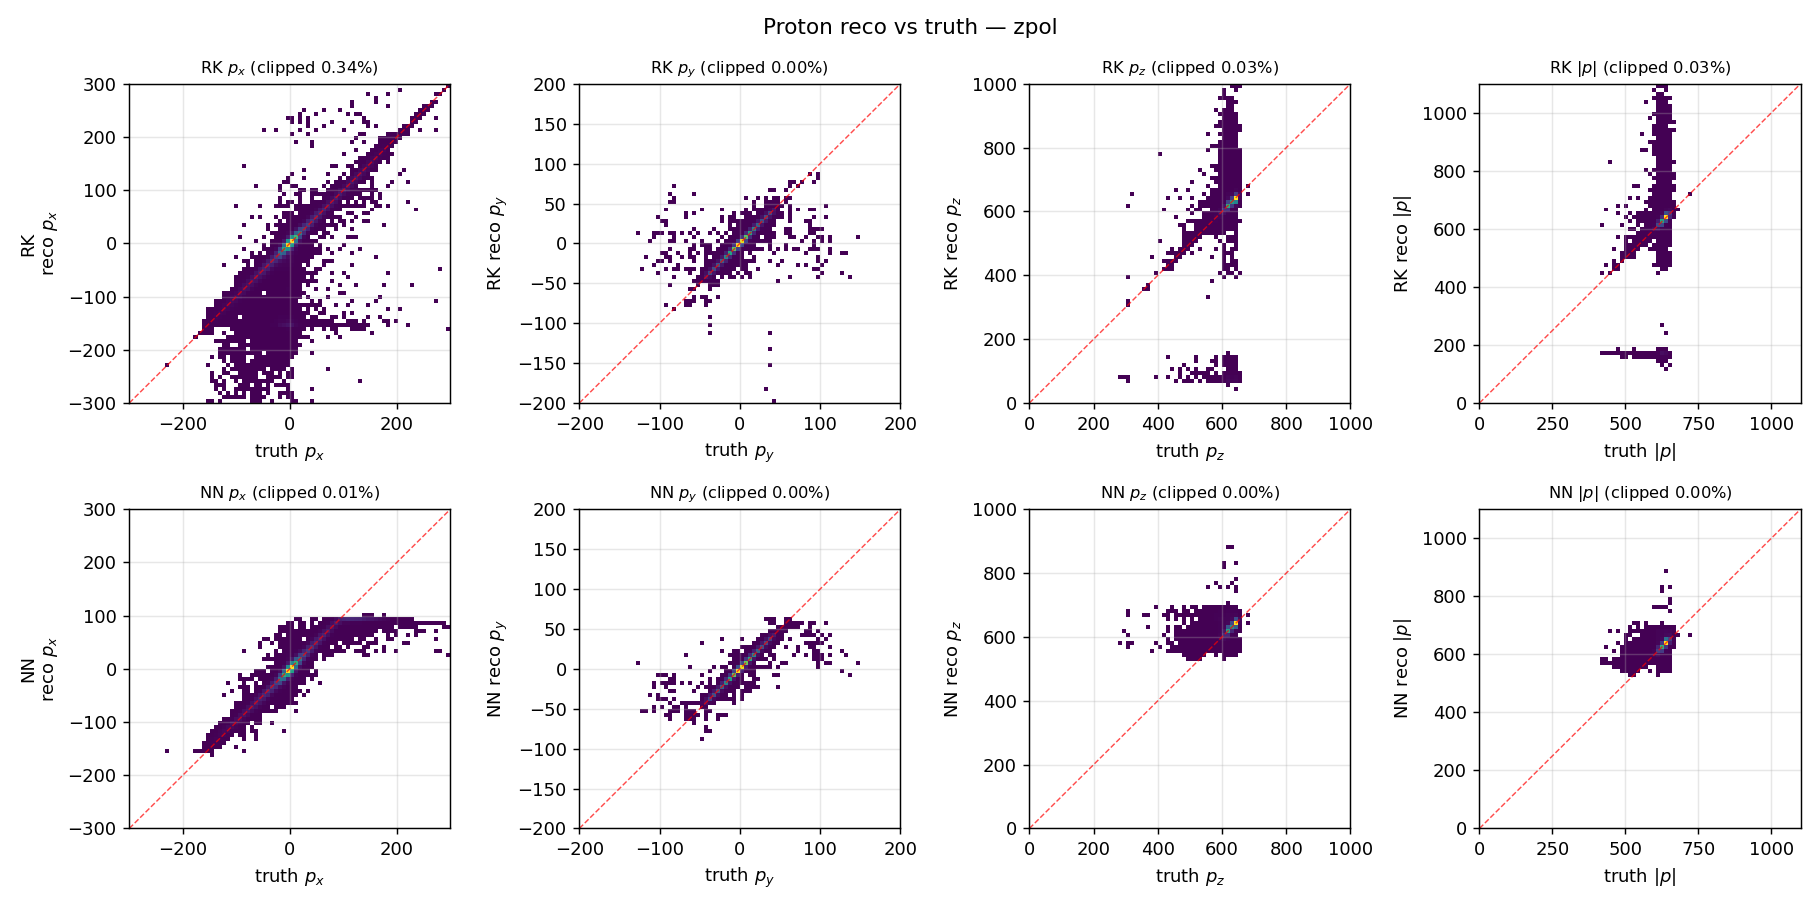
\includegraphics[width=0.95\textwidth]{figures/rk_vs_nn_breakup/proton_reco_vs_truth_zpol.png}
\caption{质子 reco vs truth 2D 散点, zpol。}
\end{figure}

\subsection{Per-event 一致性 (RK vs NN)}
对每个事件, 比较 $|p_{RK}-p_{truth}|$ 与 $|p_{NN}-p_{truth}|$。$y=x$ 线下方为 RK 更接近 truth 的事件, 上方为 NN 更接近 truth 的事件。

\begin{figure}[h]\centering
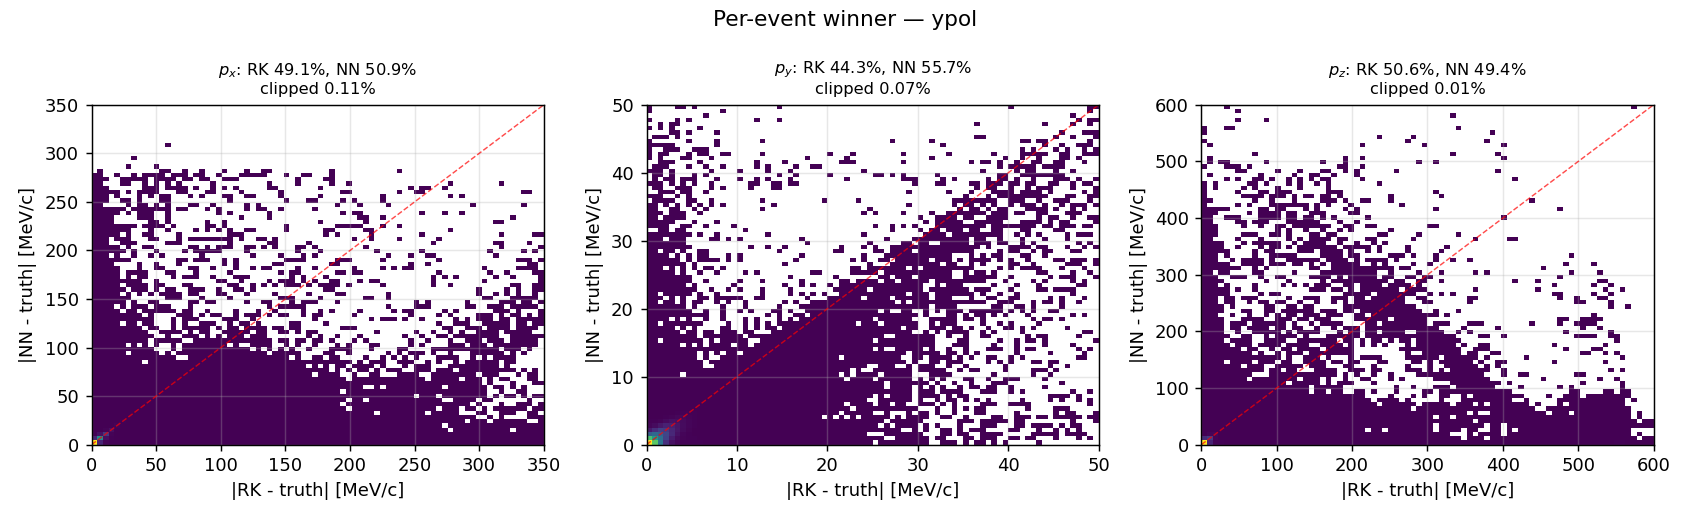
\includegraphics[width=0.95\textwidth]{figures/rk_vs_nn_breakup/proton_per_event_winner_ypol.png}
\caption{Per-event winner, ypol。}
\end{figure}

\begin{figure}[h]\centering
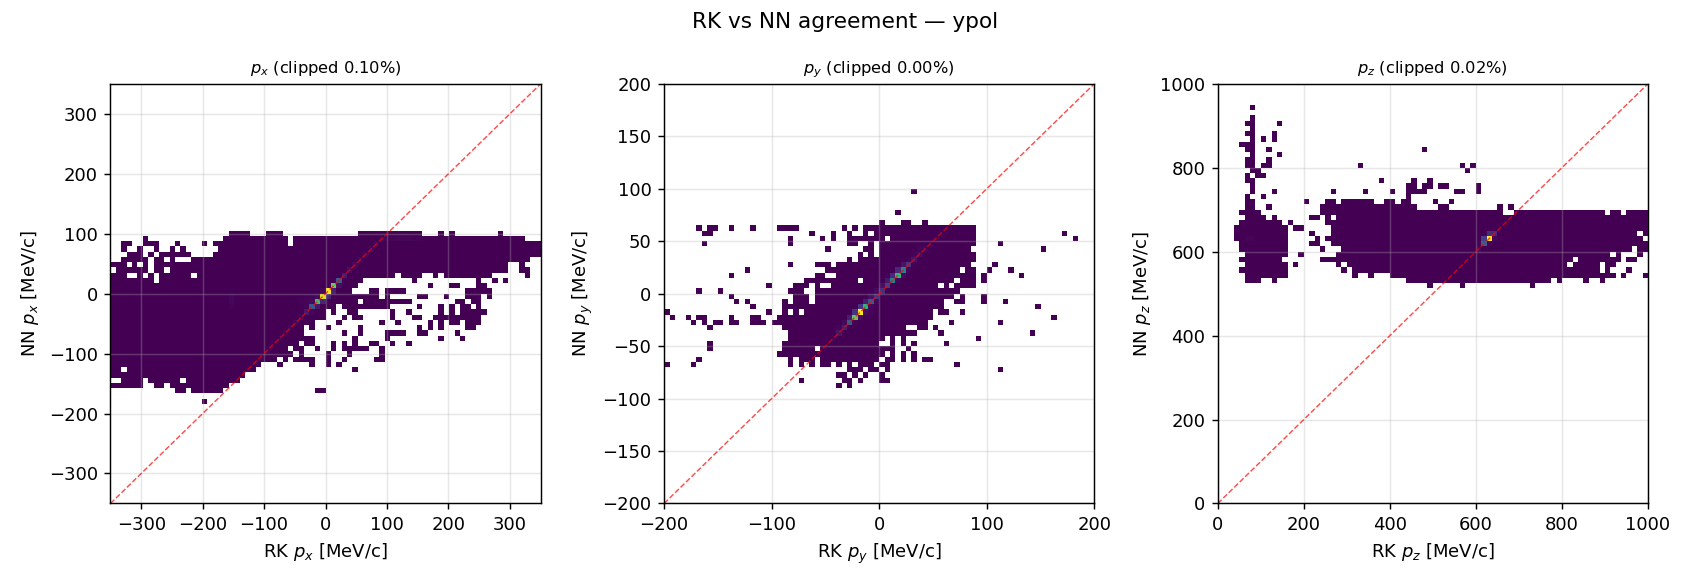
\includegraphics[width=0.95\textwidth]{figures/rk_vs_nn_breakup/proton_rk_vs_nn_agreement_ypol.png}
\caption{RK vs NN 直接一致性, ypol。}
\end{figure}

\begin{figure}[h]\centering
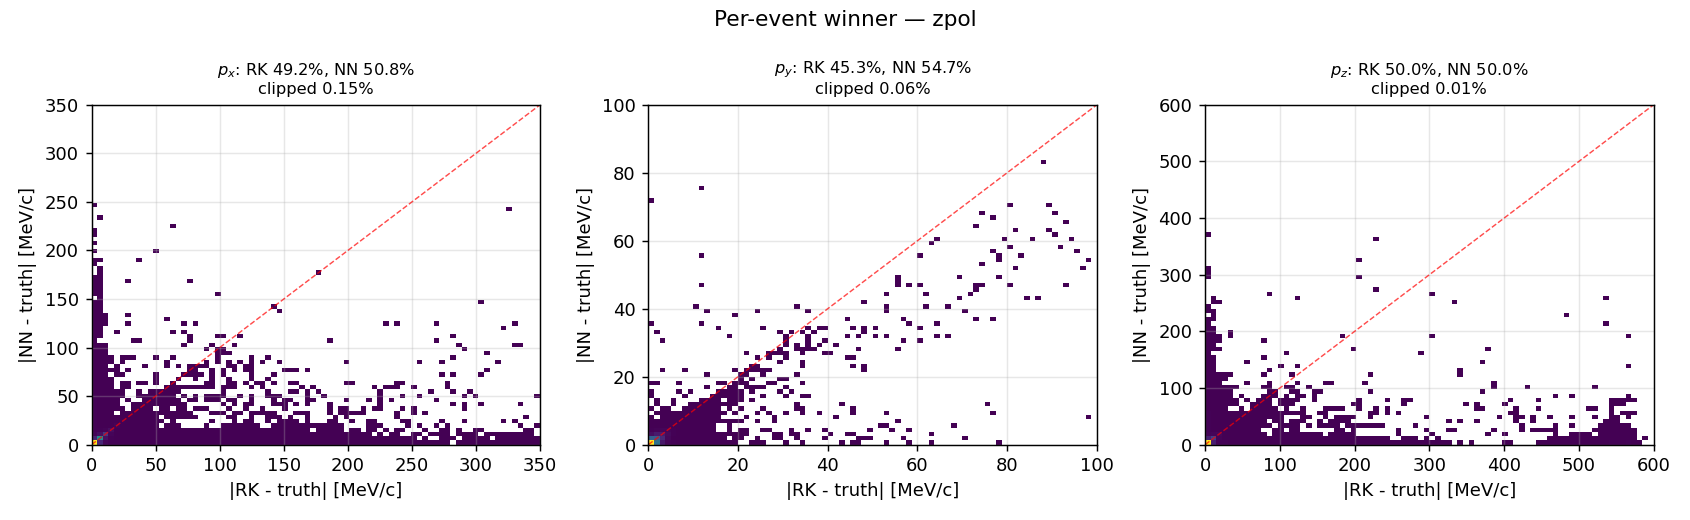
\includegraphics[width=0.95\textwidth]{figures/rk_vs_nn_breakup/proton_per_event_winner_zpol.png}
\caption{Per-event winner, zpol。}
\end{figure}

\begin{figure}[h]\centering
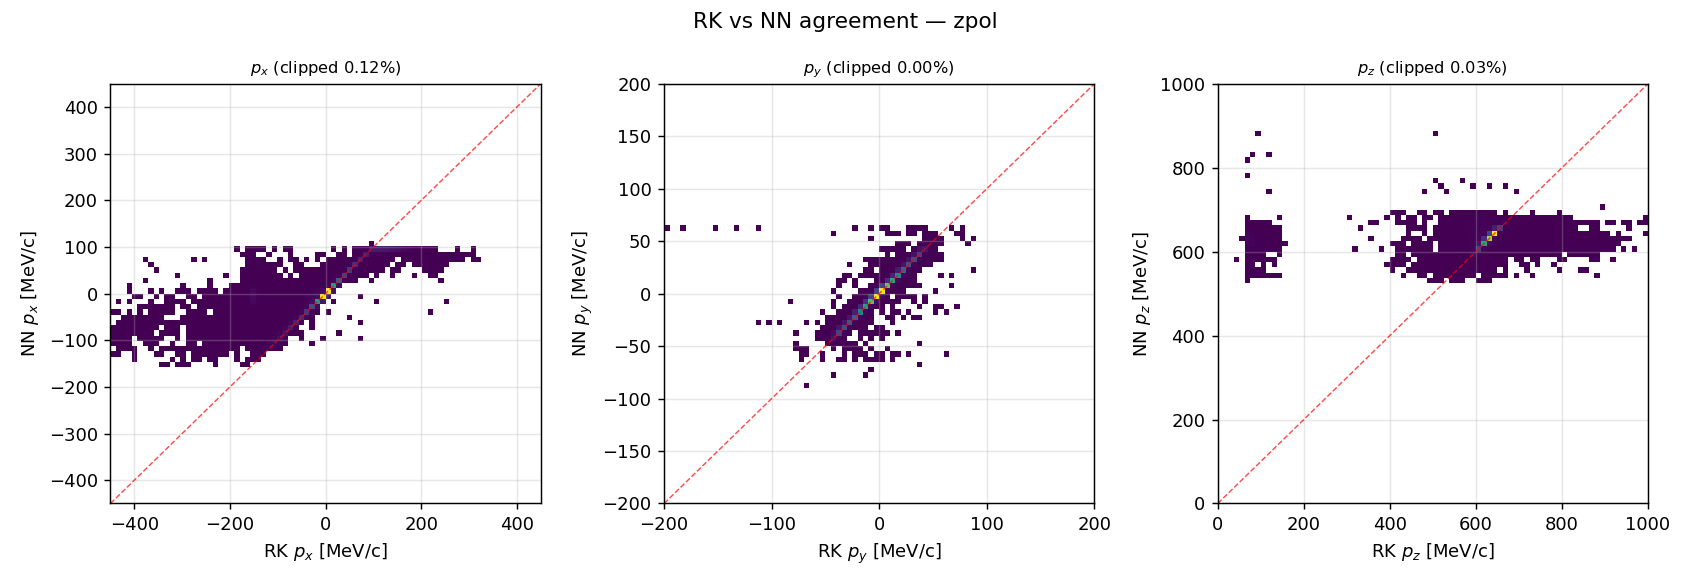
\includegraphics[width=0.95\textwidth]{figures/rk_vs_nn_breakup/proton_rk_vs_nn_agreement_zpol.png}
\caption{RK vs NN 直接一致性, zpol。}
\end{figure}

\subsection{Per-cell 分布}
\begin{figure}[h]\centering
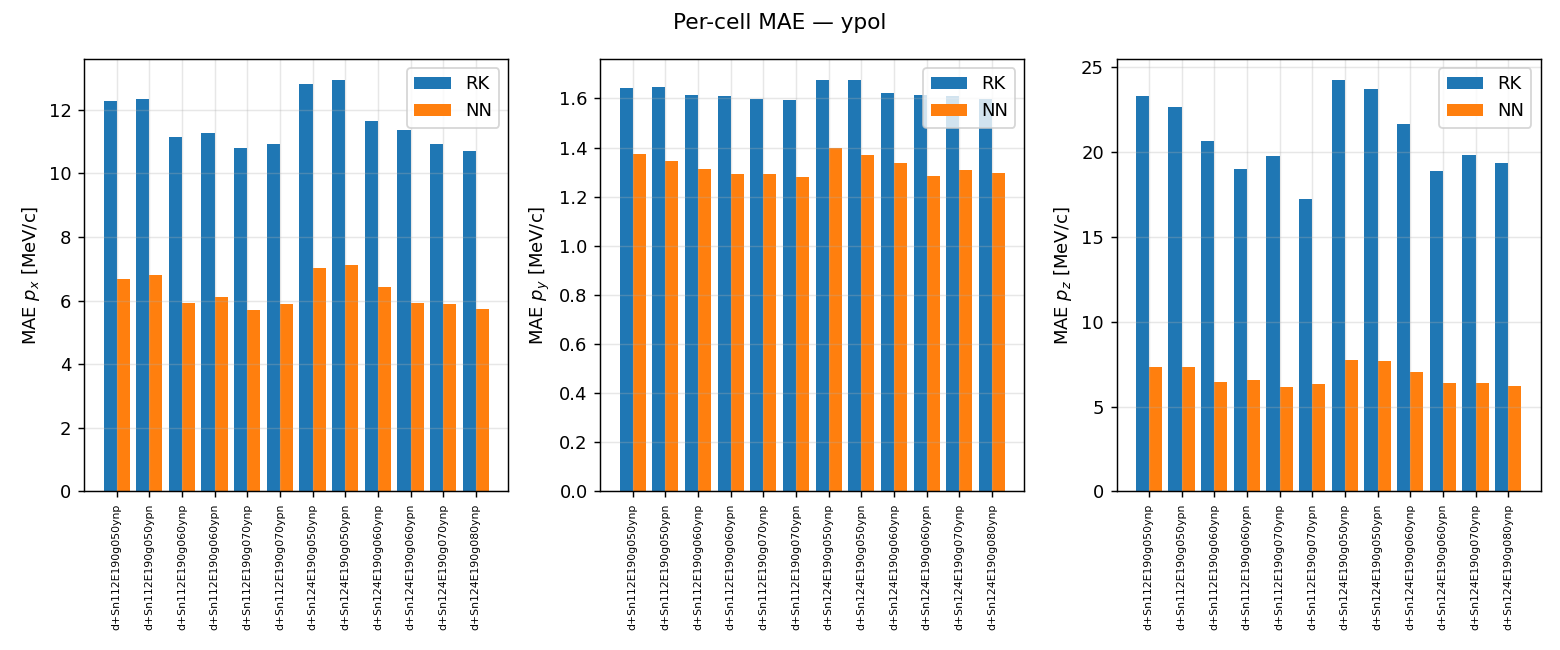
\includegraphics[width=0.95\textwidth]{figures/rk_vs_nn_breakup/proton_per_cell_mae_ypol.png}
\caption{Per-cell MAE, ypol。}
\end{figure}

\begin{figure}[h]\centering
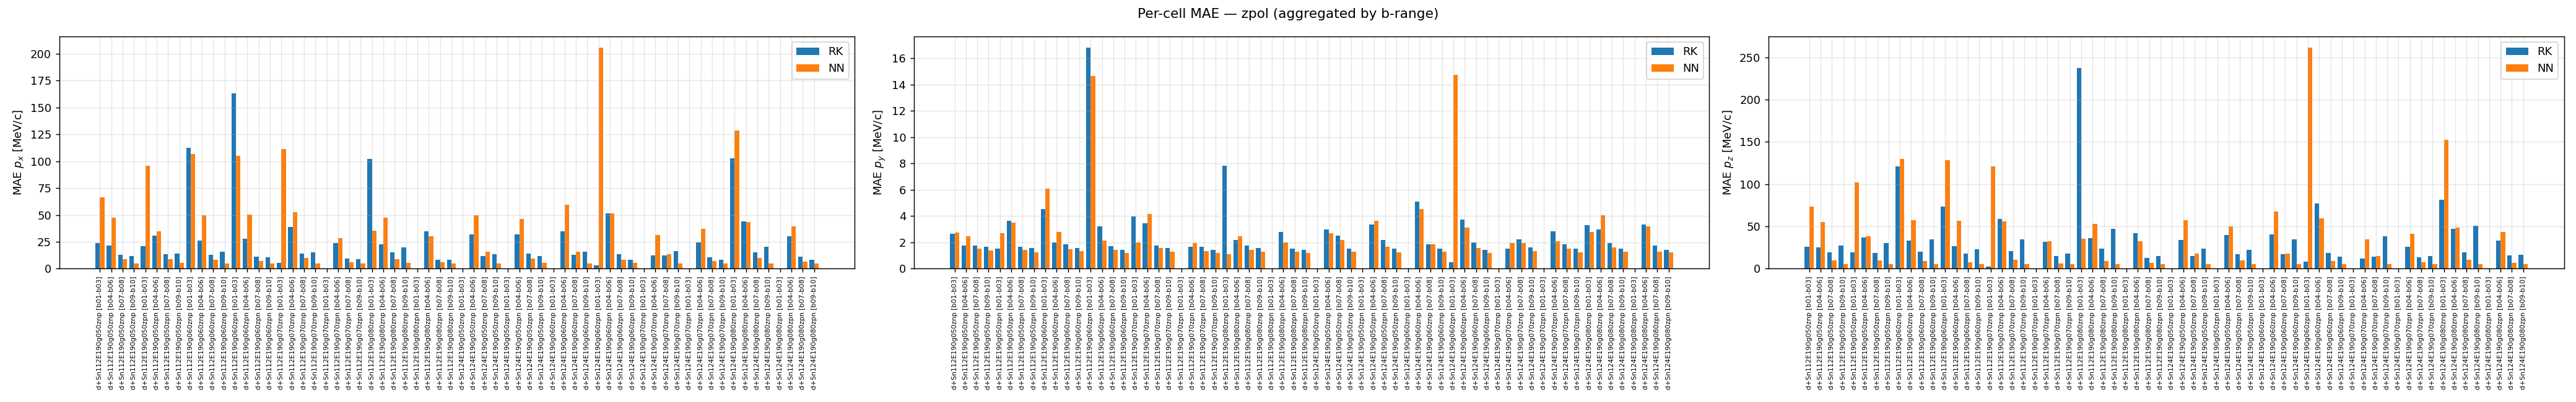
\includegraphics[width=0.95\textwidth]{figures/rk_vs_nn_breakup/proton_per_cell_mae_zpol.png}
\caption{Per-cell MAE, zpol (按 b-range 聚合)。}
\end{figure}

\begin{figure}[h]\centering
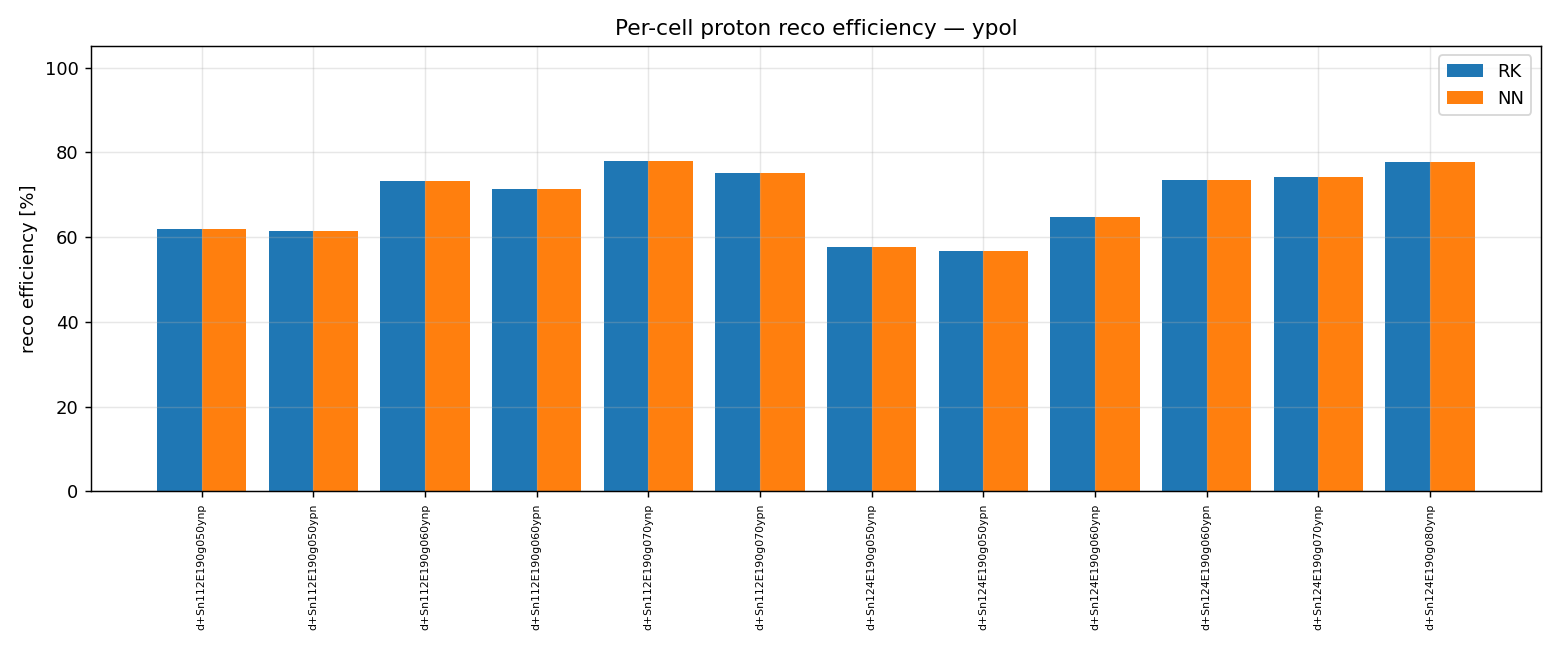
\includegraphics[width=0.95\textwidth]{figures/rk_vs_nn_breakup/proton_efficiency_per_cell_ypol.png}
\caption{Per-cell 质子重建效率, ypol。}
\end{figure}

\begin{figure}[h]\centering
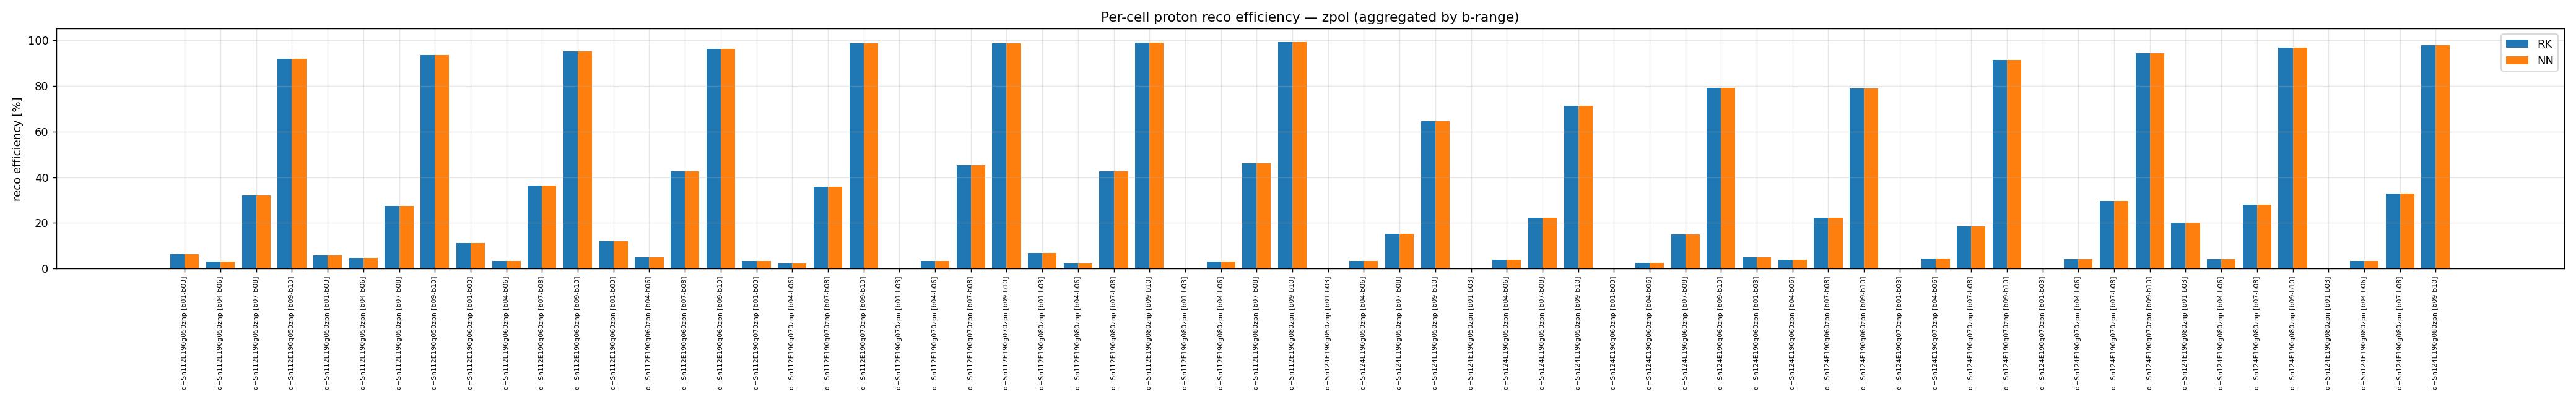
\includegraphics[width=0.95\textwidth]{figures/rk_vs_nn_breakup/proton_efficiency_per_cell_zpol.png}
\caption{Per-cell 质子重建效率, zpol (按 b-range 聚合)。}
\end{figure}

\subsection{RK 不确定度校准 (pull)}
Pull $= (|p|_{RK} - |p|_{truth}) / \sigma_p$。若 Fisher 不确定度校准良好, 应近似 $\sim\mathcal{N}(0,1)$。

\begin{figure}[h]\centering
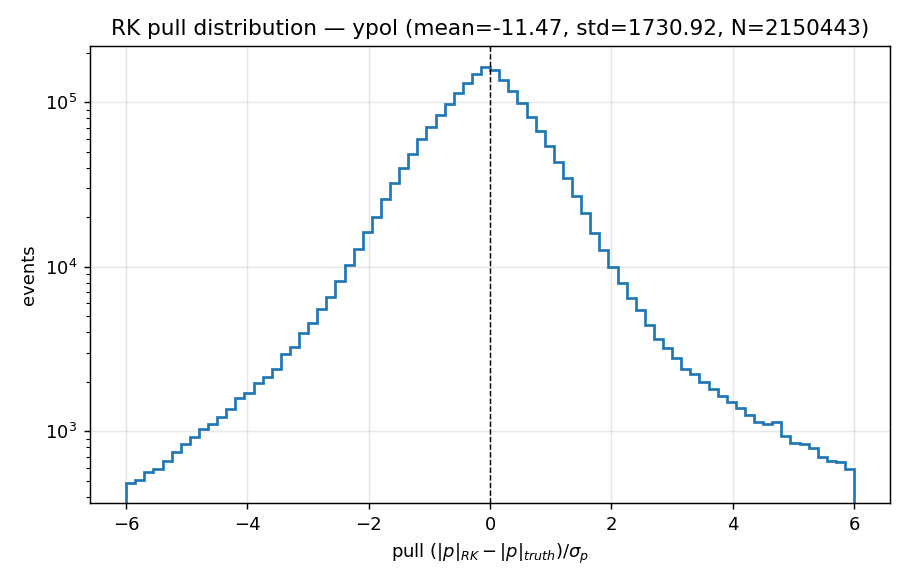
\includegraphics[width=0.7\textwidth]{figures/rk_vs_nn_breakup/proton_rk_pull_ypol.png}
\caption{RK pull 分布, ypol。}
\end{figure}

\begin{figure}[h]\centering
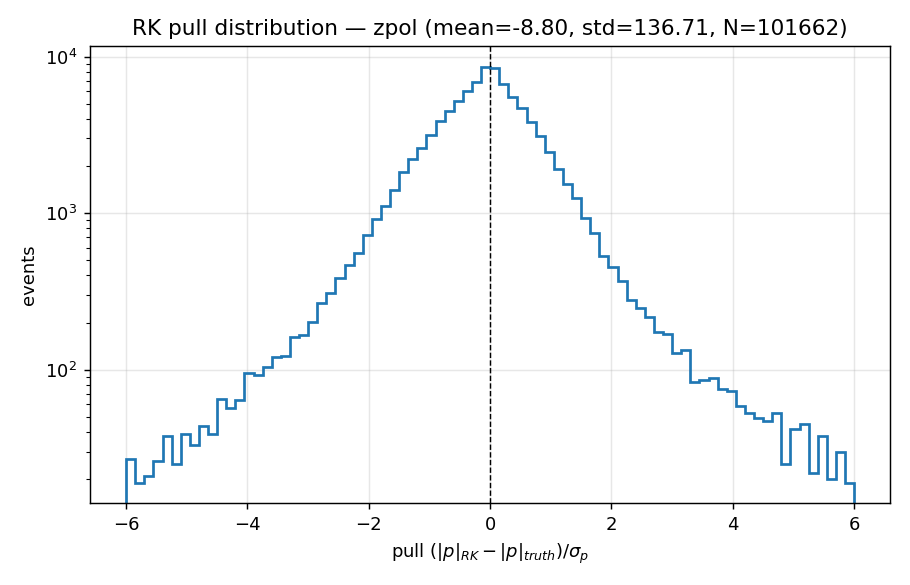
\includegraphics[width=0.7\textwidth]{figures/rk_vs_nn_breakup/proton_rk_pull_zpol.png}
\caption{RK pull 分布, zpol。}
\end{figure}

\section{中子重建 --- truth vs reco}
中子动量在 RK 和 NN 后端中均由 NEBULA $\beta$-method 重建 (后端选择只影响质子重建)。下方残差为单后端 (使用 NN 文件)。

\begin{figure}[h]\centering
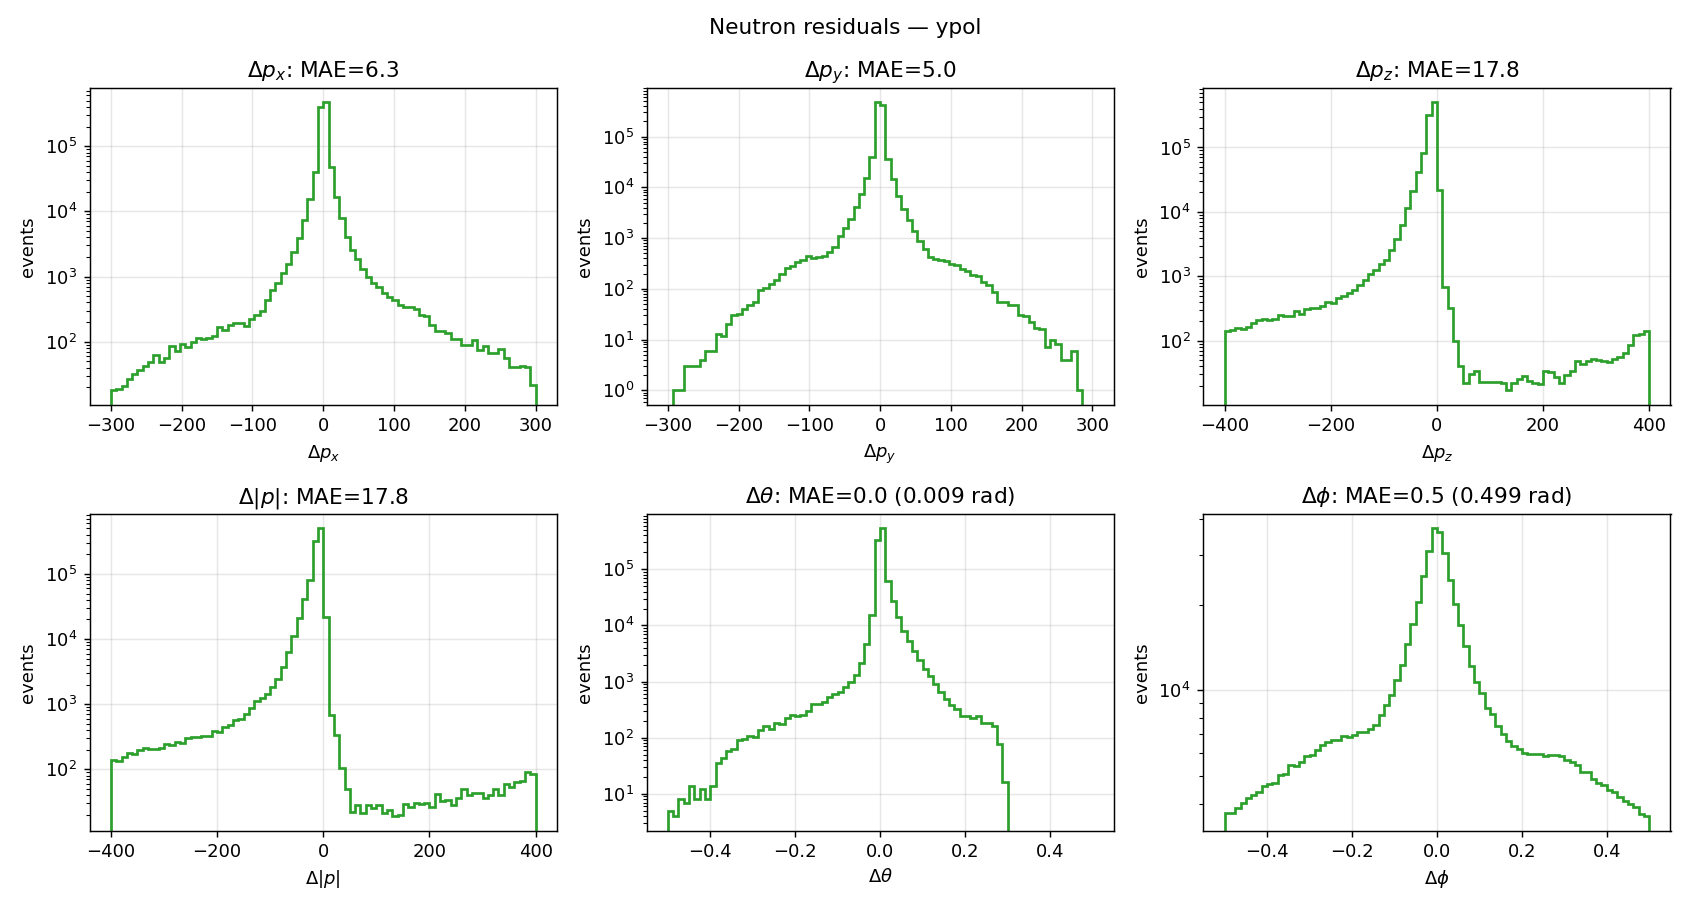
\includegraphics[width=0.95\textwidth]{figures/rk_vs_nn_breakup/neutron_residuals_ypol.png}
\caption{中子残差分布, ypol。}
\end{figure}

\begin{figure}[h]\centering
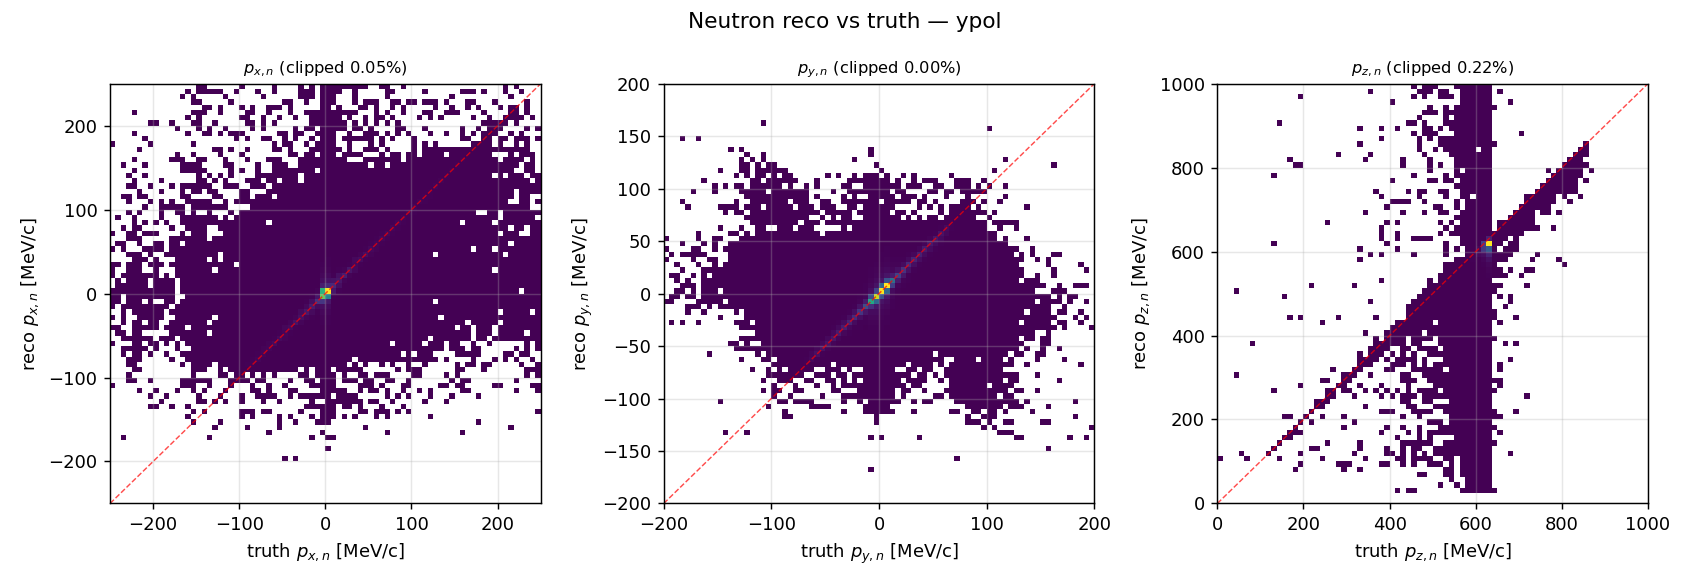
\includegraphics[width=0.95\textwidth]{figures/rk_vs_nn_breakup/neutron_reco_vs_truth_ypol.png}
\caption{中子 reco vs truth 2D 散点, ypol。}
\end{figure}

\begin{figure}[h]\centering
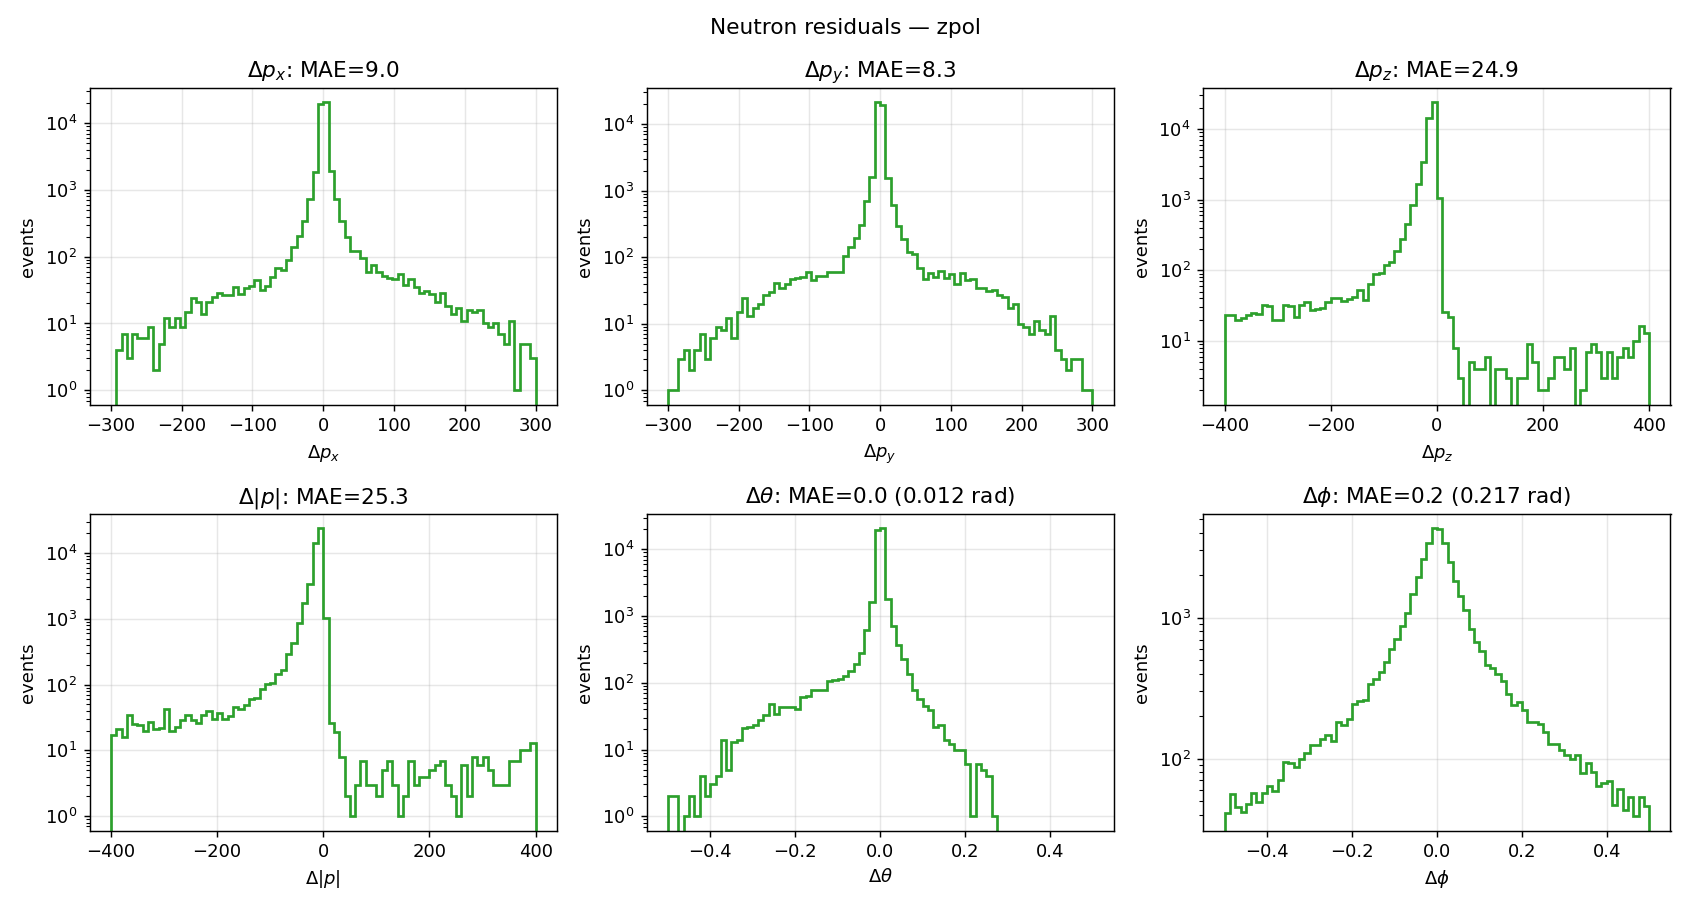
\includegraphics[width=0.95\textwidth]{figures/rk_vs_nn_breakup/neutron_residuals_zpol.png}
\caption{中子残差分布, zpol。}
\end{figure}

\begin{figure}[h]\centering
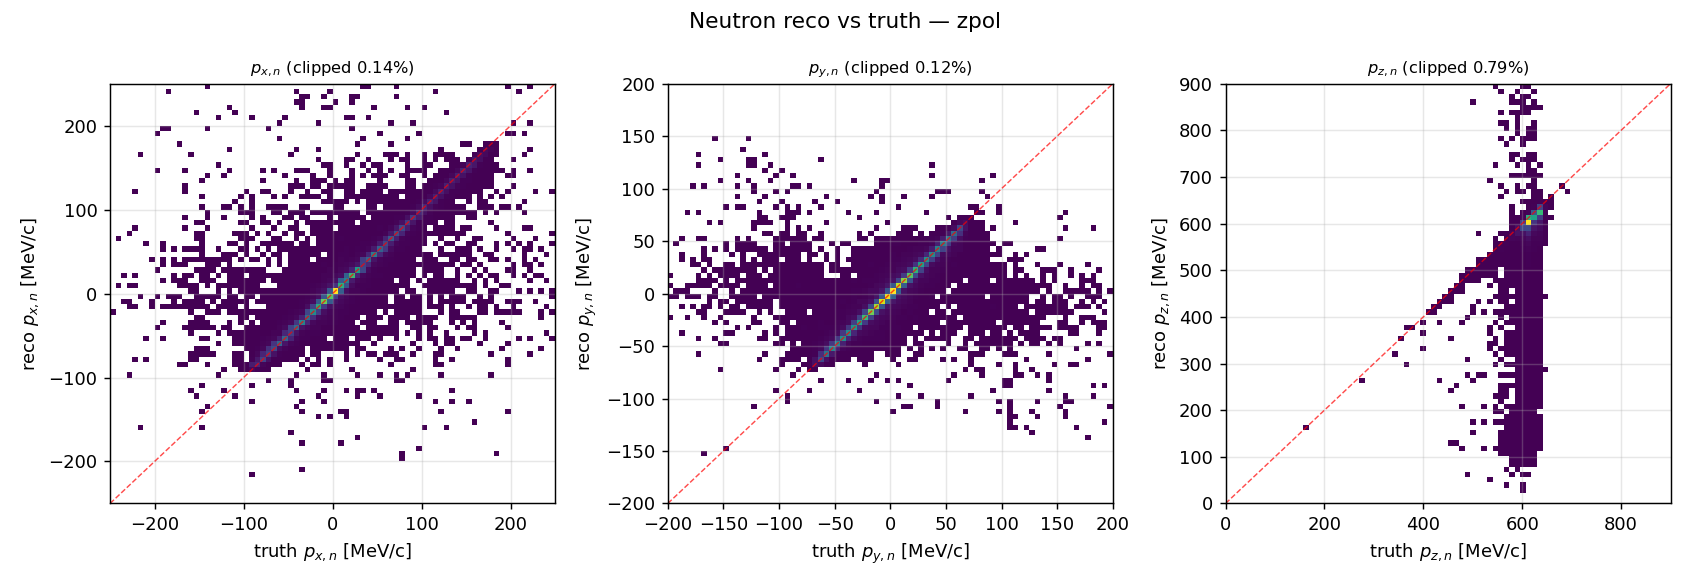
\includegraphics[width=0.95\textwidth]{figures/rk_vs_nn_breakup/neutron_reco_vs_truth_zpol.png}
\caption{中子 reco vs truth 2D 散点, zpol。}
\end{figure}

\section{结论}
(运行 pipeline 后填入。)

\appendix
\section{Per-cell 数值表}
(完整 per-cell 数值见 \texttt{summary.json}。)

\end{document}
